\section{Implementation}

\subsection{Coherence Optimizations}

Most coherence protocol do not support dynamically selecting coherence optimizations (as discussed in \cref{related_work}).
Spandex \cite{Spandex} is one which does, and dynamic coherence optimizations have already been suggested in prior work \cite{dynamic_cache_coherence}.

In Spandex, there are four states: \textit{Invalid}, \textit{Valid} (read-only copy expecting self-invalidation), \textit{Shared} (read-only copy expecting writer-invalidation), and \textit{Owned} (writable with no invalidation messages).

To limit the scope of coherence optimizations, we will consider the special case of producer/consumer relationships, where the producer issues and completes all stores before the consumer issues and completes all loads every epoch, and this pattern repeats. This is a widespread paradigm in pipelined parallelism, such as recurrent neural net training and inference.

\textbf{MESI:} In MESI, initially all lines would be invalid-state. The producer's first store to a line issues an invalidation on the bus and moves the line into modified-state. Subsequent stores hit. The consumer's first load to a line requests this line from the producer, moving both copies into shared-state.

\textbf{Spandex:} Without optimization, the Spandex coherence protocol emulates this, except the L2 is directory-based not bus-based, so the invalidation request looks up any processors which hold the line.

\textbf{Spandex Producer-Owned:} One possible optimization is to have the producer always own the buffer, so all of its stores hit locally. The consumer would have to look the line up in the producer's cache, but the owner can be predicted in hardware (suggested in \cite{dynamic_cache_coherence}), so this request goes from L1-to-L1 (bypassing the L2).
%\footnote{One may be concerned about memory consistency, if data can change while the consumer is loading it. Such a program would already have synchronization forcing the producer to `happen-before' the consumer to be correct in the first place. This existing synchronization is sufficient to maintain memory consistency. Waiting on this synchronization not limit the degree of parallelism, because th producer can be working on a second input datum in a double-buffered fashion.}
The compiler would insert a self-invalidation request in the consumer's code at the end of every epoch, to maintain memory consistency.
This is optimal when the loads are sparse, because traffic is only generated for each load.

\textbf{Spandex Consumer-Owned:} Another possible optimization is to have the consumer always own the buffer, so all of its loads hit locally, as suggested in \cite{dynamic_cache_coherence}. The producer would writethrough with owner prediction, allowing it to send data directly to the consumer's cache.
This is optimal when the write are sparse, because traffic is only generated for each write and there is little memory parallelism. No computation of the producer is logically dependent on store, but much of the consumer's computation may be logically dependent on the result of a load, so increasing the latency of stores in exchange for decreasing the latency of loads can be desirable.

\subsection{Identifying Producer/Consumer Relationships}

In order to identify the memory access pattern among multiple parallel tasks, we need an Intermediate Representation (IR) that takes task-level parallelism into account. Traditional compiler IRs like LLVM \cite{LLVM} and GIMPLE \cite{GIMPLE} do not support this, for example. HPVM is an extension of LLVM that represents task- and data-parallelism \cite{HPVM}. Currently, HPVM programs are written in C with library calls, which is a cumbersome interace, but there are plans to add a frontend to higher-level languages such as Keras.

In HPVM, programs are represented as a hierarchical dataflow graph (DFG). Every node is either called a `leaf' or an `internal' node. For example in \cref{fig:hierarchical_dfg} C, E, and F are leaves, while A, B and D are internal.

Leaf nodes can contain computation while internal nodes can only string together other nodes. HPVM can execute one input at a time, in which case the parallelism is the width of the DFG, but HPVM  also supports `streaming' (pipelined) execution, where time can be divided into epochs where every node runs once each epoch and the parallelism is the number of nodes in the DFG. In each epoch, every node runs on its own data-item, passing data to its successors to compute on in the next epoch. The data passed through pointers between nodes every epoch is exactly the kind of repeated producer/consumer relationship that we want to optimize.

We want to detect any loads and stores in different nodes that refer to the same memory location. Therefore, we trace each pointer from its definition to its use.
Initially, our pass will assign all producer/consumer memory accesses to a given coherence optimization.
In the future, our compiler-pass would examine the memory access-pattern on these pointers.

\subsection{Access-Pattern Analysis}

HPVM gives us a hierarchical DFG graph (see \cref{fig:hierarchical_dfg}). The first step is to flatten the graph, so we see how data is passed between the leaves (see \cref{fig:flattened_dfg}). This is done by \cref{algo:flatten_dfg}. 

\begin{figure}[h]
    \centering
    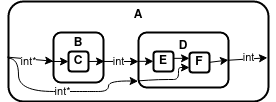
\includegraphics[width=0.45\textwidth]{hierarchical_dfg.png}
    \caption{Hierarchical DFG}
    \Description{Letters are nodes. At the first level, A contains B and D. At the second level, B contains C (leaf), while D contains E (leaf) and F (leaf).}
    \label{fig:hierarchical_dfg}
\end{figure}

\begin{algorithm}[h]
%\SetAlgoLined
\SetKwInOut{Input}{input}
\SetKwInOut{Output}{output}

\SetKwData{hdfg}{hdfg}
\SetKwData{fdfg}{fdfg}
\SetKwData{source}{source}
\SetKwData{destination}{destination}

\Input{a hierarchical DFG, \hdfg}
\Output{a flat DFG, \fdfg}
 \For{\source in \hdfg nodes}{
  \eIf{\source is leaf}{
    \(\source' := \source\)
  }{
    \(\source' := \source.\mathrm{entry}\), where \source.{entry} is a dummy node bearing that name. It will be removed later.\;
  }
  \For{\destination, where \(\source \to \destination\) in \hdfg}{
    \eIf{\destination is leaf}{
      \(\destination' := \destination\)\;
    }{
      \(\destination' := \destination.\mathrm{entry}\)\;
    }
    Insert \(\source' \to \destination'\) into \fdfg\;
  }
 }
 \caption{Flattening the HPVM DFG}
 \label{algo:flatten_dfg}
\end{algorithm}

\begin{figure}[h]
    \centering
    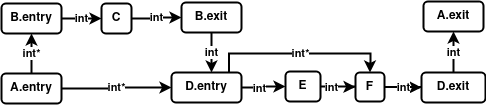
\includegraphics[width=0.49\textwidth]{flattened_dfg.png}
    \caption{Flattened DFG}
    \Description{A.entry to B.entry to C to B.exit to D.entry to F to E to D.exit to A.exit. In parallel, A.entry to D.entry. In parallel, D.entry to E}
    \label{fig:flattened_dfg}
\end{figure}

Next, we need to expose the leaf-connectivity (see \cref{fig:leaf_dfg}), because the leaves are the nodes which contain all computation, including loads and stores. This is done by \cref{algo:leafen_dfg}.

\begin{algorithm}[h]
%\SetAlgoLined
\SetKwInOut{Input}{input}
\SetKwInOut{Output}{output}

\SetKwData{ldfg}{ldfg}
\SetKwData{fdfg}{fdfg}
\SetKwData{node}{node}
\SetKwData{predecessor}{predecessor}
\SetKwData{successor}{successor}

\Input{a flat DFG, \fdfg}
\Output{a leaf DFG, \ldfg}
Initialize \ldfg to a copy of \fdfg\;
\For{\node \(\in\) \fdfg}{
  \If{\node is not a leaf and not the root entry/exit}{
    \For{\(\predecessor \to \node, \node \to \successor \in \ldfg\)}{
      Remove \(\predecessor \to \node\) from \ldfg\;
      Remove \(\node \to \successor\) from \ldfg\;
      Insert \(\predecessor \to \successor\) into \ldfg\;
    }
  }
}
\caption{Pruning non-leaves from the flat DFG}
\label{algo:leafen_dfg}
\end{algorithm}

\begin{figure}[h]
    \centering
    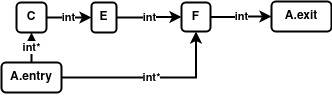
\includegraphics[width=0.4\textwidth]{leaf_dfg.png}
    \caption{Leaf Dataflow Graph}
    \label{fig:leaf_dfg}
\end{figure}

Finally, we need to look through the leaf DFG and determine where there is implicit memory communication (see the memory communication graph in \cref{fig:mem_comm_dfg}). This is done by \cref{algo:mem_comm_dfg}.

\begin{algorithm}[h]
%\SetAlgoLined
\SetKwInOut{Input}{input}
\SetKwInOut{Output}{output}

\SetKwData{ldfg}{ldfg}
\SetKwData{mcdfg}{mcdfg}
\SetKwData{node}{node}
\SetKwData{A}{A}
\SetKwData{B}{B}
\SetKwData{predecessor}{predecessor}
\SetKwData{successor}{successor}

\Input{a leaf DFG, \ldfg}
\Output{a memory-communication DFG, \mcdfg}

Initialize \ldfg to a copy of \mcdfg\;
\For{\(\node \in \ldfg\)}{
  \If{\node emits a pointer type}{
    \For{\(\node \to \A, \node \to \B \in \ldfg\)}{
      \If{Pointer is writable in \A and \A precedes \B}{
        Insert \(\A \to \B\) into \mcdfg\;
      }
    }
  }
}
\caption{Pruning non-leaves from the flat DFG}
\label{algo:mem_comm_dfg}
\end{algorithm}

\begin{figure}[h]
    \centering
    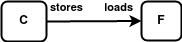
\includegraphics[width=0.3\textwidth]{mem_comm_dfg.png}
    \caption{Memory Communication Graph}
    \label{fig:mem_comm_dfg}
\end{figure}

Finally, we have analyzed the memory access-patterns in the program and identified consumer/producer relationships for cache optimization. Future work would do even more analysis on these relationships.